\section{Conclusion}
\label{sec:conclusion}

All things considered, an audio amplifier with the smallest number of components that allows a greater gain in voltage was the main objective of this laboratory. A theoretically and simulated model was created to analyze this amplifier and see how it works. \par
Using Octave as the theoretical analysis and Ngspice for the simulation, a very discrepant results were observed between the two. The main cause of this problem is due of the transistor models used in Ngspice that is more complex than Octave models. Transistors in Ngspice makes it impossible to get the same results because of non-linearity components.\par
It is possible to say that the theoretical model had a good result even with its low complexity, but only for low frequencies, as shown in figures~\ref{fig:SIM_OUT}, \ref{fig:SIM_PH}, \ref{fig:MAT_OUT}, \ref{fig:MAT_PH}. This is possibly due to the rise of second and higher order derivatives of the function that describe the circuit and in the theoretical analysis are not considered. The phasor calculation are, however, diferent in all frequencies. But it shows that Ngspice has results more like reality due to more accurate models and components.

The tables with the results are the following:

%%	DC

\begin{table}[h]
\centering
\begin{minipage}[t]{0.35\linewidth}
 	 \begin{tabular}[t]{|l|r|}
 	   \hline    
 	   {\bf Name} & {\bf Value} \\ \hline
 	   \input{../mat/MAT_DC_tab}
 	 \end{tabular}
\end{minipage}
\begin{minipage}[t]{0.40\linewidth}
  	\begin{tabular}[t]{|l|r|}
    	\hline    
   		{\bf Name} & {\bf Value} \\ \hline
    	\input{../sim/SIM_DC_tab}
  	\end{tabular}
\end{minipage}

  	\caption{Results in Octave and NGSpice, respectivily. The variables are of type {\it voltage} and expressed in Volt (As shown in Tables \ref{tab:TEO_DC} and \ref{tab:SIM_DC}).}
\end{table}

%%	Impedance

\begin{table}[h]
\centering
\begin{minipage}[t]{0.47\linewidth}
 	 \begin{tabular}[t]{|l|r|}
 	   \hline    
 	   {\bf Name} & {\bf Value} \\ \hline
 	   \input{../mat/MAT_IMP_tab}
 	 \end{tabular}
\end{minipage}
\begin{minipage}[t]{0.47\linewidth}
  	\begin{tabular}[t]{|l|r|}
    	\hline    
   		{\bf Name} & {\bf Value} \\ \hline
    	\input{../sim/SIM_ZIN_tab}
  	\end{tabular}
	\begin{tabular}[t]{|l|r|}
    	\hline    
   		{\bf Name} & {\bf Value [A or V]} \\ \hline
    	\input{../sim/SIM_ZOUT_tab}
  	\end{tabular}
\end{minipage}

\caption{Results in Octave and NGSpice, respectivily. NGSpice values are of of type {\it impedance} and expressed in Ohm; variables preceded by \# are of type {\it impedance} and expressed in Ohm; other variables are adimentional. (As shown in Tables \ref{tab:TEO_IMP}, \ref{tab:SIM_ZIN} and \ref{tab:SIM_ZOUT})}
\end{table}

%%	AC

\begin{table}[h]
\centering
\begin{minipage}[t]{0.40\linewidth}
 	 \begin{tabular}[t]{|l|r|}
 	   \hline    
 	   {\bf Name} & {\bf Value} \\ \hline
 	   \input{../mat/MAT_GAIN_tab}
 	 \end{tabular}
\end{minipage}
\begin{minipage}[t]{0.45\linewidth}
  	\begin{tabular}[t]{|l|r|}
    	\hline    
   		{\bf Name} & {\bf Value} \\ \hline
    	\input{../sim/SIM_RESULTS_tab}
  	\end{tabular}
\end{minipage}

  	\caption{Results in Octave and NGSpice, respectivily. Merit is in {\it per voltage per cost} and expressed in Volt$^{-1}$UC$^{-1}$; $f1 - f2$ is of the type {\it frequency} and expressed in Hz; other variables are adimentional. (As shown in Tables \ref{tab:TEO_RES} and \ref{tab:SIM_RES})}
\end{table}


The Merit result was 260.6748 $V^{-1}uc^{-1}$ by Ngspice. It was agreed by the members of the group that the main goal of task was completed.

\newpage
The obtained plot with NGSpice and Octave are the following:

\begin{figure}[h] \centering
	\vspace{-3cm}
	\includegraphics[height=12cm]{../sim/ampdb.pdf}
	\caption{NGSpice plot:$db(v_{out})$ and $max(db(v_{out}))-3$.}
	\label{fig:MAT_OUT}
\end{figure}

\begin{figure}[h] \centering
	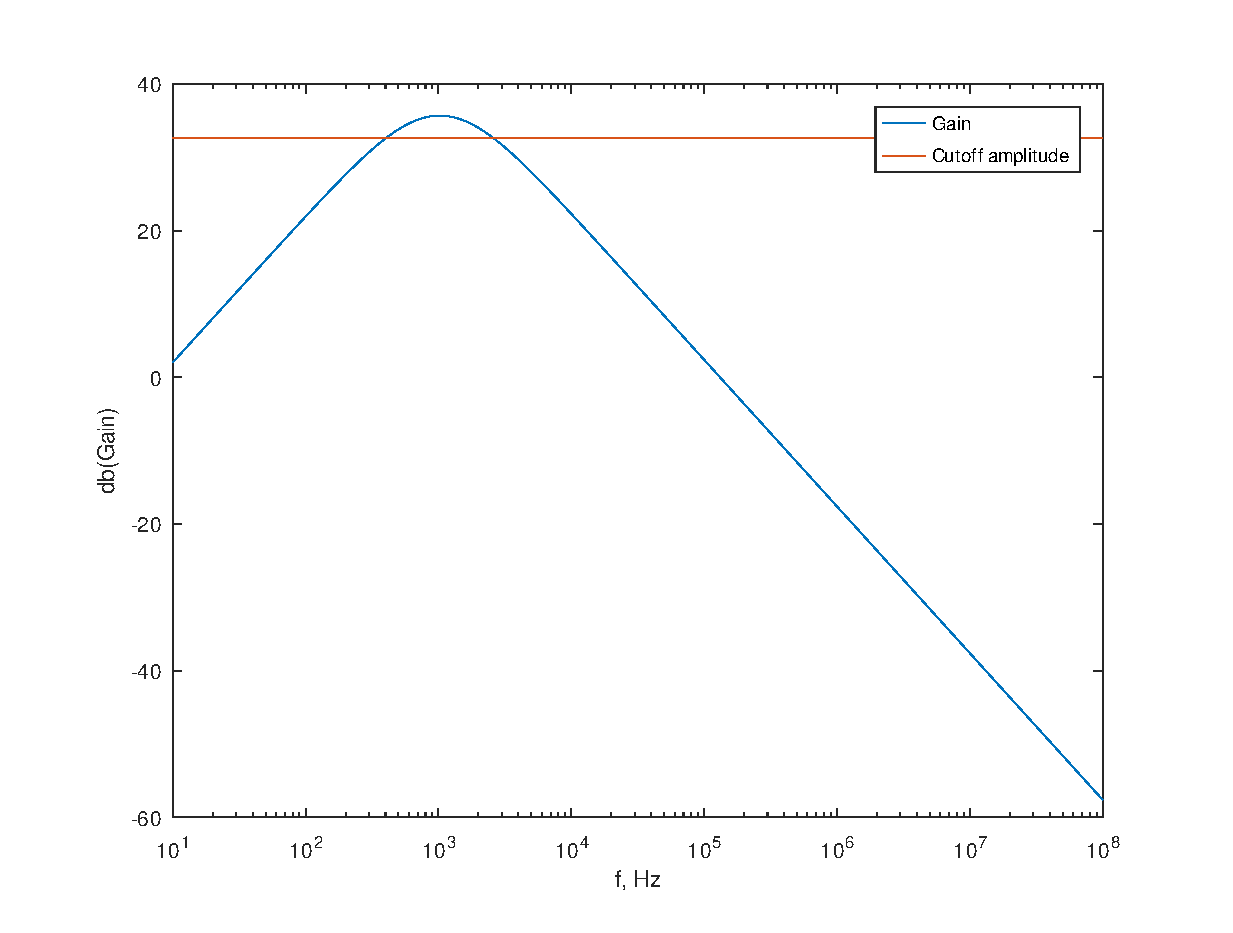
\includegraphics[height=8cm]{MAT_AB_AMP.eps}
	\caption{Octave plot:$db(v_{out})$ and $max(db(v_{out}))-3$.}
	\label{fig:SIM_OUT}
\end{figure}

\newpage

\begin{figure}[h] \centering
	\vspace{-3cm}
	\includegraphics[height=12cm]{../sim/phdb.pdf}
	\caption{NGSpice plot: Phasor of $v_{out}$, rad}
	\label{fig:MAT_PH}
\end{figure}

\begin{figure}[h] \centering
	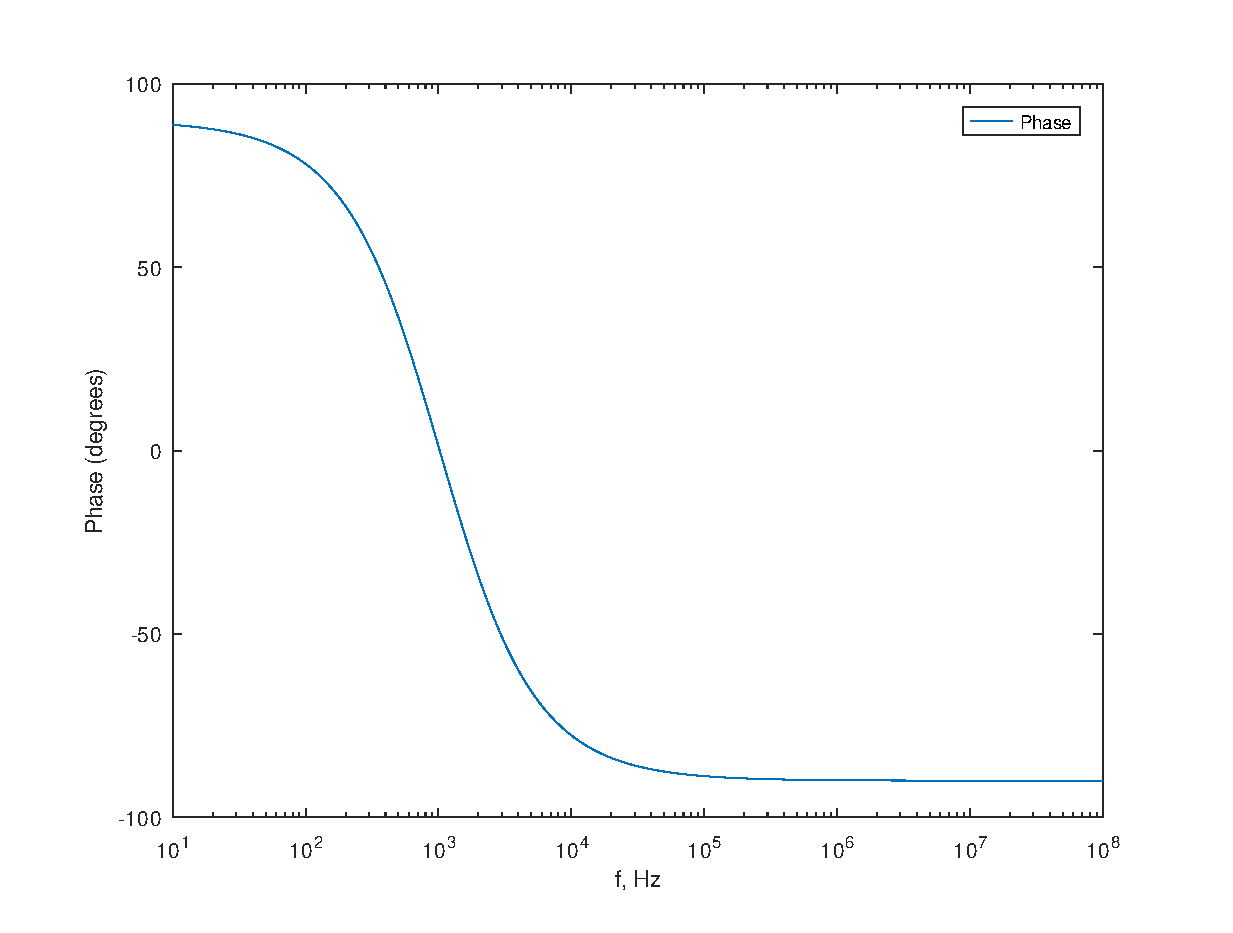
\includegraphics[height=8cm]{MAT_AB_PH.eps}
	\caption{Octave plot: Phasor of $v_{out}$, rad}
	\label{fig:SIM_PH}
\end{figure}

\newpage

\begin{figure}[h] \centering
	\vspace{-3cm}
	\includegraphics[height=12cm]{../sim/trans.pdf}
	\caption{NGSpice plot: $v_{in}$ and $v_{out}$.}
\end{figure}

\begin{figure}[h] \centering
	\vspace{-3cm}
	\includegraphics[height=12cm]{../sim/amp.pdf}
	\caption{$ \left | v_{out}/v_{in} \right |$.}
	\vspace{-2cm}
\end{figure}
